\section{Results}\label{sec:results}

Unless stated otherwise every experiment uses randomised 300\,s flights at 40\,m/s, the default
parameters of \cref{tab:params}, and common random numbers: within an experiment, run $i$ has the
same flight and noise for every filter and configuration. $M$ is the number of Monte Carlo runs
per configuration. Brackets give 95\,\% intervals (Wilson for rates, bootstrap for RMSE).

\subsection{Study regions}\label{sec:regions}
Three $0.36^\circ\times0.36^\circ$ boxes ($\approx40\times40$\,km) were chosen with a rule fixed
before the data were examined: on a 90\,m survey of the whole island, the roughest candidate box
around Nuwara Eliya, the flattest around Anuradhapura, and around Kandy the box whose roughness is
closest to the geometric mean of the two (\cref{fig:regions,tab:regions}). No box around Kandy is
nearly as smooth as that target, so the least rough one was selected: the ``Kandy'' region is
intermediate, but closer to the rugged end. The regions differ by two orders of magnitude in the
position information one altimeter sample carries (\cref{tab:terrain}): the Fisher information
density is \TerrHillFisherDensityPerMTwo{}, \TerrKandyFisherDensityPerMTwo{} and
\TerrPlainsFisherDensityPerMTwo{}\,$\times10^{-3}$\,m$^{-2}$ for the hill country, Kandy and the
plains. The synthetic terrain used during development has a 1\,km roughness similar to the hill
country (\TerrSyntheticRoughnessOnekmM{} vs.\ \TerrHillRoughnessOnekmM{}\,m) but less than half of
its information density: smooth Gaussian hills lack the slope texture of real terrain at the
scale of a few cells --- a difference that turns out to matter for the EKF.

\begin{figure}[t]
  \centering
  \begin{subfigure}[b]{0.34\textwidth}\centering
    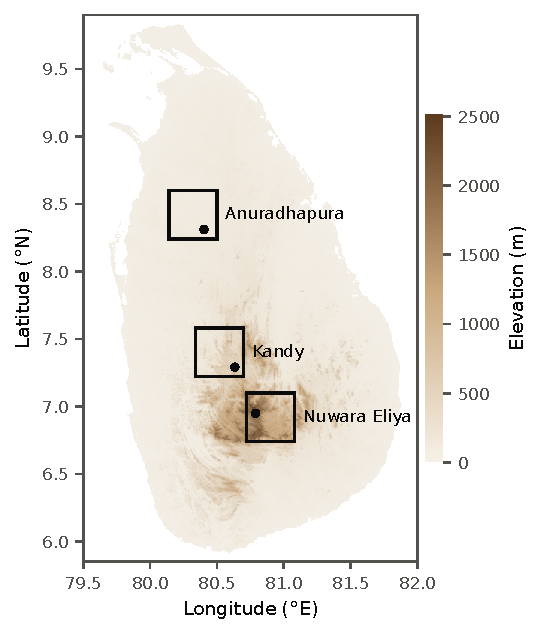
\includegraphics[width=\textwidth]{region_map.pdf}\caption{Sri Lanka (COP90 survey).}
  \end{subfigure}\hfill
  \begin{subfigure}[b]{0.64\textwidth}\centering
    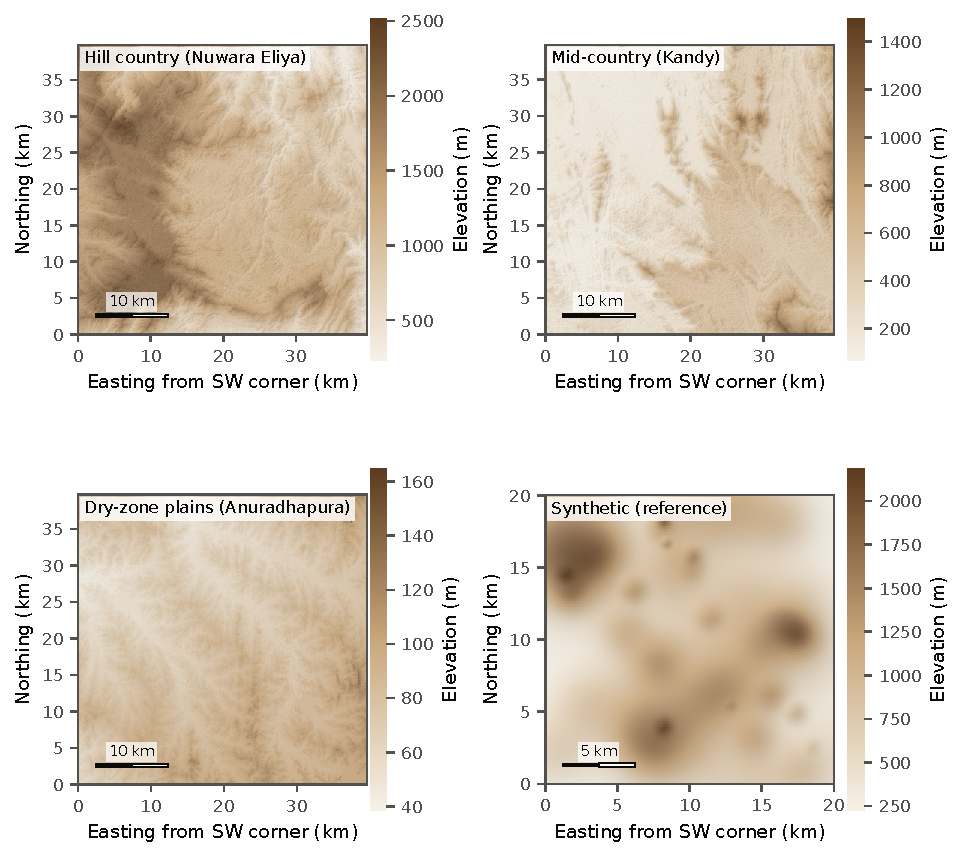
\includegraphics[width=\textwidth]{terrain_overview.pdf}\caption{The three regions and the synthetic reference.}
  \end{subfigure}
  \caption{Study regions. Boxes in (a) were selected by the pre-registered roughness rule;
    (b) shows the 30\,m Copernicus GLO-30 elevation (colour) with hillshading. Note the different
    elevation scales: the plains span only 127\,m.}\label{fig:regions}
\end{figure}

\begin{table}[t]
  \centering\small
  \caption{Study regions as requested from OpenTopography and the processed UTM grids.}\label{tab:regions}
  % Generated by scripts — do not edit.
\begin{tabular}{lrrrr}
\toprule
Region & Latitude ($^\circ$N) & Longitude ($^\circ$E) & Size (km) & Grid (30 m cells) \\
\midrule
Hill country (Nuwara Eliya) & 6.74--7.10 & 80.72--81.08 & 39.8 $\times$ 39.8 & 1327\,$\times$\,1325 \\
Mid-country (Kandy) & 7.22--7.58 & 80.34--80.70 & 39.7 $\times$ 39.8 & 1326\,$\times$\,1323 \\
Dry-zone plains (Anuradhapura) & 8.24--8.60 & 80.14--80.50 & 39.6 $\times$ 39.8 & 1325\,$\times$\,1319 \\
\bottomrule
\end{tabular}

\end{table}

\begin{table}[t]
  \centering\small
  \caption{Terrain statistics (definitions in \cref{sec:data}).}\label{tab:terrain}
  % Generated by scripts — do not edit.
\begin{tabular}{lrrrr}
\toprule
Statistic & Hill country & Kandy & Dry-zone plains & Synthetic \\
\midrule
Min.\ elevation (m) & 224 & 64 & 38 & 221 \\
Max.\ elevation (m) & 2\,521 & 1\,499 & 165 & 2\,190 \\
Elevation range (m) & 2\,297 & 1\,436 & 127 & 1\,970 \\
Elevation std (m) & 450 & 215 & 16 & 381 \\
Mean slope (\%) & 35.0 & 24.2 & 3.1 & 22.6 \\
Slope std (\%) & 21.0 & 17.6 & 2.4 & 14.7 \\
Roughness, 1 km window (m) & 64.5 & 37.7 & 3.5 & 62.7 \\
Fisher density ($10^{-3}$\,m$^{-2}$) & 13.49 & 7.38 & 0.16 & 5.63 \\
Grid (cells) & 1327\,$\times$\,1325 & 1326\,$\times$\,1323 & 1325\,$\times$\,1319 & 667\,$\times$\,667 \\
\bottomrule
\end{tabular}

\end{table}

\subsection{E1 --- When does linearisation fail?}\label{sec:e1}
\emph{Setup:} dead reckoning, EKF and particle filters with 5\,000 and 20\,000 particles on
identical flights; $\sigma_0 \in \{100, 250, 500, 1000, 1500, 2000\}$\,m on all three regions;
$M = \EOneRuns$ per cell (5\,400 flights in total).

\begin{figure}[t]
  \centering
  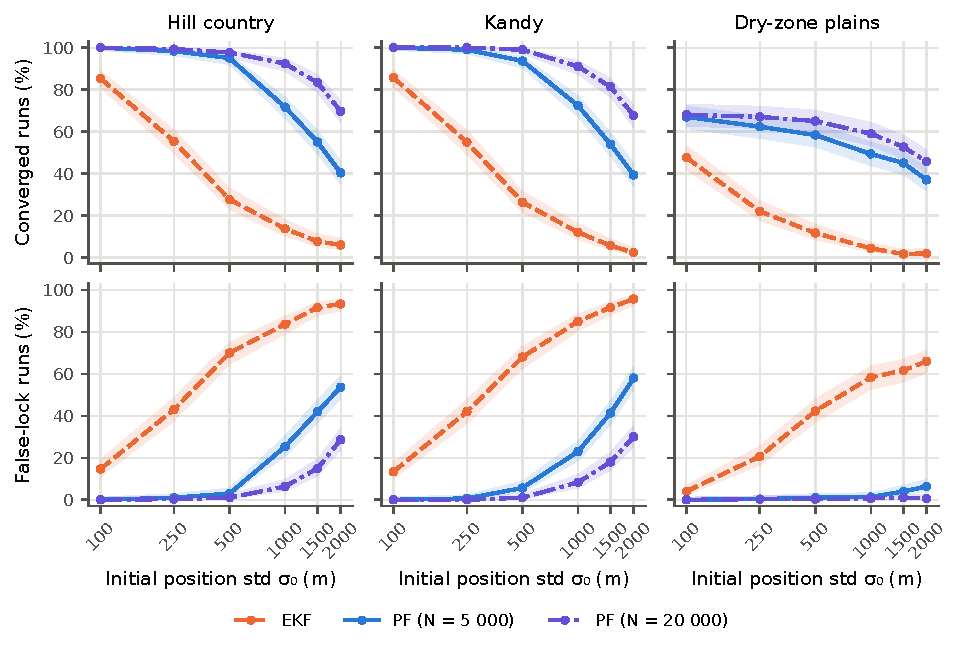
\includegraphics[width=\textwidth]{e1_rates.pdf}
  \caption{E1: share of converged (top) and falsely locked (bottom) runs against the initial
    position uncertainty, $M = \EOneRuns$ per point, Wilson 95\,\% bands. Dead reckoning never
    converges and is omitted.}\label{fig:e1rates}
\end{figure}

\begin{figure}[t]
  \centering
  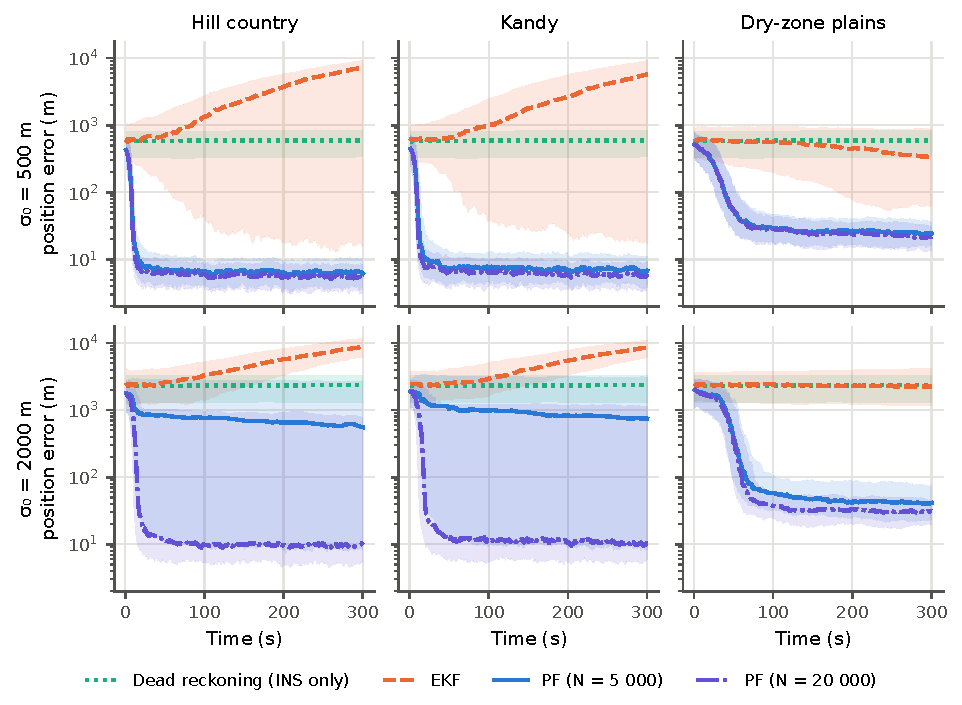
\includegraphics[width=\textwidth]{e1_error_vs_time.pdf}
  \caption{E1: median position error over time (bands: interquartile range over the
    $M = \EOneRuns$ runs) for $\sigma_0 = 500$\,m (top) and 2\,000\,m (bottom). Log scale.}\label{fig:e1time}
\end{figure}

\Cref{fig:e1rates} answers the question directly, and the answer depends strongly on the
terrain. On the hill country the EKF fails even when the initial error is small: at
$\sigma_0 = 100$\,m it converges in only \EOneHillSOneZeroZeroEkfConv\,\% of the runs and
falsely locks in \EOneHillSOneZeroZeroEkfFl\,\%; at 500\,m it converges in
\EOneHillSFiveZeroZeroEkfConv\,\% and is confidently wrong in \EOneHillSFiveZeroZeroEkfFl\,\%. The
particle filters converge in \EOneHillSFiveZeroZeroPfFiveZeroZeroZeroConv\,\% ($N=5\,000$) and
\EOneHillSFiveZeroZeroPfTwoZeroZeroZeroZeroConv\,\% ($N=20\,000$) of the same runs. Paired over the
runs, the PF converges significantly more often than the EKF in every one of the 18 cells
(McNemar, all $p < 10^{-10}$; \cref{tab:e1tests} in the appendix). This is a much earlier failure
than on the smooth synthetic terrain, where the EKF had held up to $\sigma_0 = 1$\,km during
development: the real DEM's slope changes within a few cells, so the one-cell Jacobian is already
wrong when the error is a few tens of metres. The Kandy region behaves almost identically.

\Cref{fig:e1time} shows how the EKF fails. Its median error \emph{grows} during the flight and
ends well above the dead-reckoning error on both hilly regions: corrections computed from the
wrong slope also corrupt the bias estimate, so the EKF drifts faster than the uncorrected INS.
A linearised terrain filter is worse than no terrain aiding at all once its linearisation is
invalid.

The particle filter's limit is different. Its error drops within 10--20\,s to a few metres, and
it degrades gracefully with $\sigma_0$: at 2\,km the filter with 20\,000 particles still converges in
\EOneHillSTwoZeroZeroZeroPfTwoZeroZeroZeroZeroConv\,\% of the runs, the one with 5\,000 in
\EOneHillSTwoZeroZeroZeroPfFiveZeroZeroZeroConv\,\%. Its failures are almost all false locks
(\EOneHillSTwoZeroZeroZeroPfFiveZeroZeroZeroFl\,\% and
\EOneHillSTwoZeroZeroZeroPfTwoZeroZeroZeroZeroFl\,\%): with a wide prior, few particles start
close enough to the truth, and the cloud collapses onto another patch whose profile matches.
More particles help significantly from $\sigma_0 \ge 500$\,m on every region.

The flat plains tell the opposite story about failure. No filter converges reliably: even at
$\sigma_0 = 100$\,m the 20\,000-particle PF converges in only
\EOnePlainsSOneZeroZeroPfTwoZeroZeroZeroZeroConv\,\% of the runs, and in
\EOnePlainsSTwoZeroZeroZeroPfTwoZeroZeroZeroZeroConv\,\% at 2\,km. Yet it almost never locks
falsely (\EOnePlainsSTwoZeroZeroZeroPfTwoZeroZeroZeroZeroFl\,\% at 2\,km): it knows that it does
not know. Its covariance stays wide, and its median error still falls from 500\,m to about 25\,m
within the first 100\,s, because even 3\,m of roughness is not zero information; most of its
``non-converged'' runs end just above the 50\,m threshold rather than lost (\cref{sec:e2}). The
EKF on the plains, by contrast, is falsely locked in \EOnePlainsSFiveZeroZeroEkfFl\,\% of the runs
at $\sigma_0 = 500$\,m. In the tracking phase
of converged runs the PF's RMSE is \EOneHillSFiveZeroZeroPfTwoZeroZeroZeroZeroTrack\,m (hill
country), \EOneKandySFiveZeroZeroPfTwoZeroZeroZeroZeroTrack\,m (Kandy) and
\EOnePlainsSFiveZeroZeroPfTwoZeroZeroZeroZeroTrack\,m (plains) at $\sigma_0 = 500$\,m
(\cref{tab:e1track} in the appendix).

The corridor rule for the altitude puts the UAV up to \EOneRadarHillMax\,m above the terrain on
the hill country (median of the per-flight maximum \EOneRadarHillMedian\,m); a range-independent
3\,m radar noise is optimistic at such ranges, which is a limitation of the sensor model
(\cref{sec:limitations}).

\subsection{E2 --- Terrain informativeness}\label{sec:e2}
\emph{Setup:} EKF and PF ($N = 5\,000$), $\sigma_0 = 500$\,m, $M = \ETwoRuns$ random flights
per region. For every flight the terrain under the true track is characterised by its mean 1\,km
roughness and by the terrain information $\sum_k |\nabla h(\pv_k)|^2/\sigma_z^2$, split into
along- and cross-track components.

\begin{figure}[t]
  \centering
  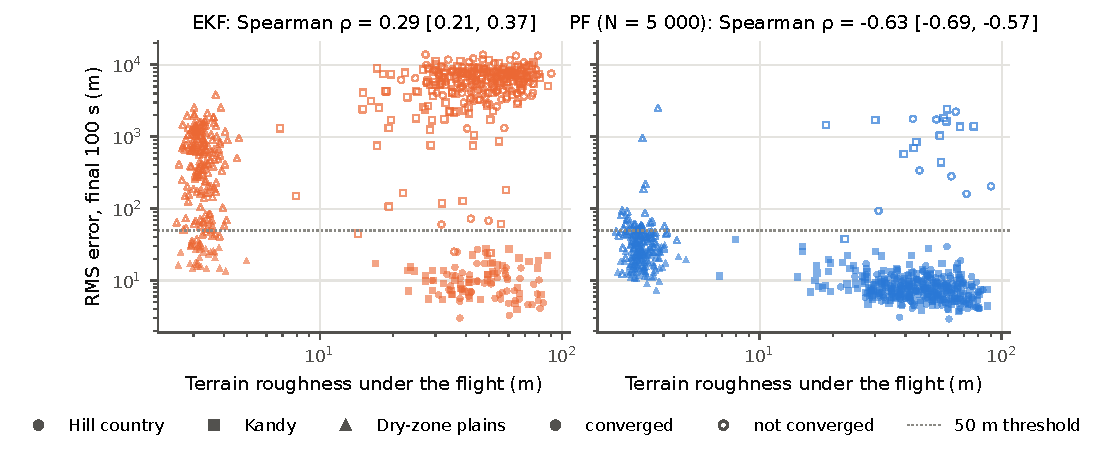
\includegraphics[width=\textwidth]{e2_scatter.pdf}
  \caption{E2: RMS error over the final 100\,s of each flight against the roughness of the
    terrain under that flight ($M = \ETwoRuns$ per region, $\sigma_0 = 500$\,m). Spearman rank
    correlation with bootstrap 95\,\% CI over all flights.}\label{fig:e2scatter}
\end{figure}

\Cref{fig:e2scatter} relates each flight's final error to the terrain it crossed. For the particle
filter, rougher terrain means smaller error (Spearman $\rho = \ETwoRhoPfFiveZeroZeroZero$
[$\ETwoRhoPfFiveZeroZeroZeroLo$, $\ETwoRhoPfFiveZeroZeroZeroHi$]). For the EKF the correlation has
the \emph{opposite} sign ($\rho = \ETwoRhoEkf$ [$\ETwoRhoEkfLo$, $\ETwoRhoEkfHi$]): the same texture that informs
the particle filter breaks the EKF's linearisation, so its failures concentrate on the most
informative terrain. Within a single region the correlations are weak (PF $\rho$ between
\ETwoPlainsPfFiveZeroZeroZeroRho{} and \ETwoKandyPfFiveZeroZeroZeroRho), i.e.\ most of the effect
is between terrain types rather than between flights over the same type. Binned by the terrain
information collected along the flight (\cref{fig:e2binned}), the PF's convergence rate rises
from about one half on the least informative flights to over 90\,\% on the hills.

\begin{figure}[t]
  \centering
  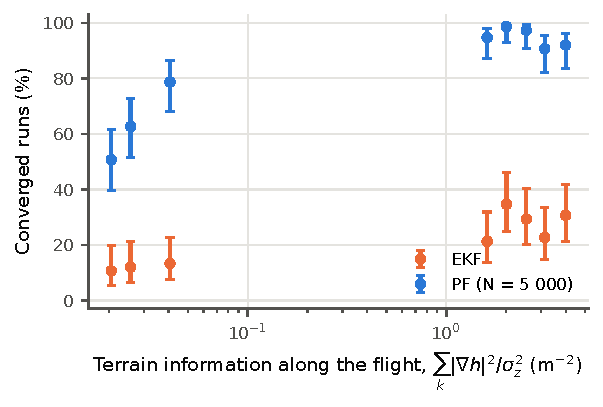
\includegraphics[width=0.62\textwidth]{e2_binned.pdf}
  \caption{E2: convergence against the terrain information along the flight (eight equal-count
    bins pooled over the three regions; Wilson 95\,\% intervals). No flight falls between the
    plains and the hills, hence the gap.}\label{fig:e2binned}
\end{figure}

Decomposing the tracking error into along- and cross-track components (\cref{tab:e2}) shows no
systematic anisotropy: the PF's along/cross RMS is \ETwoHillPfFiveZeroZeroZeroAlong{}/%
\ETwoHillPfFiveZeroZeroZeroCross\,m on the hill country, \ETwoKandyPfFiveZeroZeroZeroAlong/%
\ETwoKandyPfFiveZeroZeroZeroCross\,m around Kandy and \ETwoPlainsPfFiveZeroZeroZeroAlong/%
\ETwoPlainsPfFiveZeroZeroZeroCross\,m on the plains, and the along- and cross-track terrain
information is balanced on average (ratio $\approx 1$). The expected elongation of the error along
ridges and valleys does not appear in these averages: the 25$^\circ$ heading weave and the varied
ridge directions inside 40\,km boxes mix the two directions. The hypothesis is therefore not
supported at the ensemble level; it may still hold for individual straight flights along a valley,
which this design does not isolate.

\begin{table}[t]
  \centering\small
  \caption{E2 per region ($\sigma_0 = 500$\,m, $M = \ETwoRuns$): convergence, median roughness
    under the flights, tracking RMS along and across the track (converged runs), median ratio of
    along- to cross-track terrain information, and the within-region Spearman correlation between
    roughness and final error.}\label{tab:e2}
  % Generated by scripts — do not edit.
\begin{tabular}{llrrrrrr}
\toprule
Region & Filter & Conv.\ (\%) [95\% CI] & Rough.\ (m) & Along RMS (m) & Cross RMS (m) & $I_\parallel/I_\perp$ & $\rho_S$ \\
\midrule
Hill country & EKF & 26 [21, 33] & 48.3 & 7.6 & 8.0 & 1.01 & -0.07 \\
Hill country & PF (N = 5 000) & 96 [92, 98] & 48.3 & 6.0 & 6.0 & 1.01 & -0.16 \\
Kandy & EKF & 26 [21, 33] & 41.6 & 9.5 & 9.5 & 0.97 & 0.16 \\
Kandy & PF (N = 5 000) & 94 [89, 96] & 41.6 & 7.4 & 7.5 & 0.97 & -0.26 \\
Dry-zone plains & EKF & 12 [9, 18] & 3.2 & 14.7 & 17.5 & 1.03 & -0.07 \\
Dry-zone plains & PF (N = 5 000) & 60 [53, 67] & 3.2 & 14.7 & 15.4 & 1.03 & -0.05 \\
\bottomrule
\end{tabular}

\end{table}

\subsection{E3 --- Particle-filter design}\label{sec:e3}
\emph{Setup:} hill country, $\sigma_0 = 1$\,km, $M = \EThreeRuns$; one design parameter varied at
a time from the defaults (systematic resampling, $\tau = 0.5$, $K = 0$).

\begin{figure}[t]
  \centering
  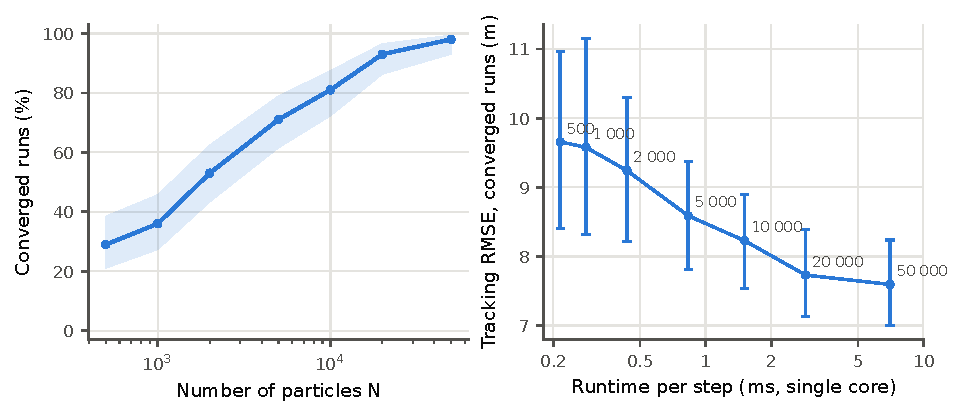
\includegraphics[width=\textwidth]{e3_particles.pdf}
  \caption{E3: convergence against the number of particles (left) and tracking RMSE of converged
    runs against the runtime per step from the single-core benchmark (right, labelled with $N$);
    $M = \EThreeRuns$, hill country, $\sigma_0 = 1$\,km.}\label{fig:e3n}
\end{figure}

\paragraph{Number of particles.} Convergence rises from \EThreeNFiveHundredConv\,\% with 500
particles to \EThreeNFiveKConv\,\% with 5\,000 and \EThreeNFiftyKConv\,\% with 50\,000
(\cref{fig:e3n}), while the tracking RMSE improves only from \EThreeNFiveHundredTrack{} to
\EThreeNFiftyKTrack\,m. Particles buy \emph{robustness of acquisition} much more than tracking accuracy:
once locked on, 500 particles track within about 2\,m of fifty thousand. The cost is
linear in $N$; even $N = 50\,000$ needs only \EThreeNFiftyKMs\,ms per step on one core, two
orders of magnitude inside the real-time budget of a 1\,Hz altimeter.

\paragraph{Resampling.} The four schemes do not differ significantly in convergence (McNemar
$p \ge 0.15$ against systematic at both $N$; \cref{tab:e3tests}) or tracking RMSE (overlapping
intervals, \cref{fig:e3design}). The schemes do differ in what they are designed to differ in:
measured directly, the variance of the offspring counts (\cref{tab:e3var}) is
\EThreeVarMultinomialFiveK{} for multinomial (theory 1.00), \EThreeVarResidualFiveK{} for residual
(theory 0.44), \EThreeVarStratifiedFiveK{} for stratified and \EThreeVarSystematicFiveK{} for
systematic resampling --- the last equal to the minimum possible for any unbiased scheme
(\EThreeVarFloorFiveK, attained when every count is $\lfloor N w\rfloor$ or $\lceil N w\rceil$).
This matches Hol, Schön and Gustafsson~\cite{hol2006}, who found stratified and residual
resampling to have lower variance than multinomial, recommended systematic resampling for its
quality and cost, and found the effect on the estimates ``not significant''; here too the lower
resampling noise is real but small compared with the other sources of error, and systematic
resampling is also the cheapest (\cref{tab:runtime}).

\paragraph{ESS threshold.} Resampling when $\Neff$ falls below $0.1N$ to $1.0N$ (every step)
changes the number of resampling steps per flight from \EThreeEssZeroPointOneResamples{} to
\EThreeEssOnePointZeroResamples{}, but not the convergence (\EThreeEssZeroPointOneConv--%
\EThreeEssOnePointZeroConv\,\%, all $p \ge 0.5$) or the tracking error.

\paragraph{Roughening.} Roughening has by far the largest effect of the design choices
(\cref{fig:e3design}, right). A small jitter, $K = 0.05$, raises convergence from
\EThreeRoughZeroPointZeroZeroConv\,\% to \EThreeRoughZeroPointZeroFiveConv\,\% (McNemar: 24 runs
gained, 1 lost, $p < 10^{-4}$) and also lowers the tracking RMSE (\EThreeRoughZeroPointZeroFiveTrack{}
vs.\ \EThreeRoughZeroPointZeroZeroTrack\,m); $K = 0.1$ gives \EThreeRoughZeroPointOneZeroConv\,\%
and $K = 0.2$ falls back to \EThreeRoughZeroPointTwoZeroConv\,\%. With $K = 0.05$, 5\,000 particles
match 20\,000 particles without roughening at a quarter of the cost. Because the jitter is
proportional to the spread of the cloud ($\sigma_j = K E_j N^{-1/4}$), roughening acts as an
\emph{adaptive} process-noise inflation: tens of metres while the cloud is still wide, which keeps
hypotheses near the truth alive between resamplings, and negligible once the cloud has collapsed.
Too much of it blurs the information the measurements provide.

\begin{figure}[t]
  \centering
  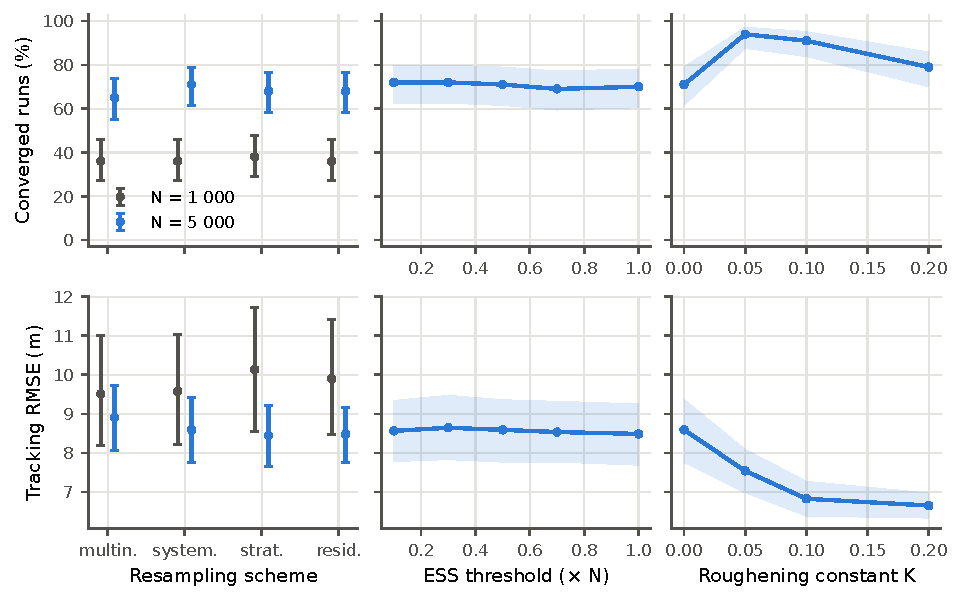
\includegraphics[width=\textwidth]{e3_design.pdf}
  \caption{E3: convergence (top) and tracking RMSE (bottom) for the resampling scheme (left,
    $N = 1\,000$ grey and 5\,000 blue), the ESS threshold (middle) and the roughening constant
    (right); $N = 5\,000$ unless stated, $M = \EThreeRuns$, 95\,\% intervals.}\label{fig:e3design}
\end{figure}

\begin{table}[t]
  \centering\small
  \caption{E3: measured variance of the offspring counts, mean over particles
    ($N_{\mathrm{eff}} \approx 0.4N$, 400 resamplings of one weight vector), with the closed forms
    for multinomial and residual resampling and the floor/ceil lower bound.}\label{tab:e3var}
  % Generated by scripts — do not edit.
\begin{tabular}{rrrrrrrr}
\toprule
$N$ & Multinomial & Systematic & Stratified & Residual & Multin.\ theory & Resid.\ theory & floor/ceil bound \\
\midrule
1\,000 & 1.001 & 0.180 & 0.269 & 0.438 & 0.997 & 0.438 & 0.179 \\
5\,000 & 1.000 & 0.179 & 0.277 & 0.442 & 1.000 & 0.441 & 0.179 \\
\bottomrule
\end{tabular}

\end{table}

\subsection{E4 --- Robustness to model mismatch}\label{sec:e4}
\emph{Setup:} hill country and Kandy (where a nominal filter converges, so there is something to
lose), $\sigma_0 = 500$\,m, $M = \EFourRuns$ per cell; the simulated world violates one model
assumption at a time while the filters keep their nominal models unless stated.

\begin{figure}[t]
  \centering
  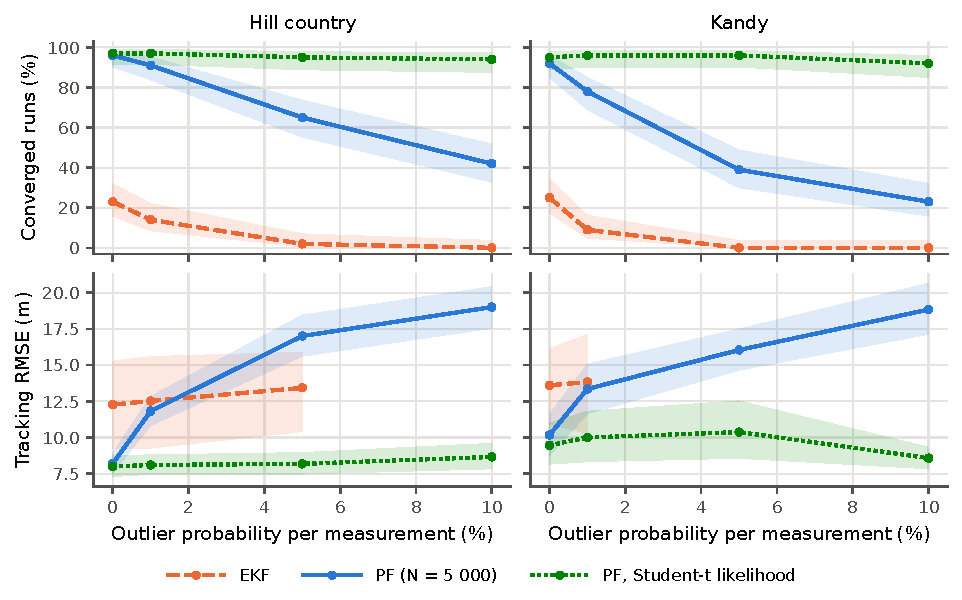
\includegraphics[width=\textwidth]{e4_outliers.pdf}
  \caption{E4: radar-altimeter outliers ($\mathcal{N}(0, 100^2)$\,m with the given probability per
    measurement). Gaussian vs.\ Student-$t$ ($\nu = 4$) likelihood; $M = \EFourRuns$, 95\,\%
    intervals.}\label{fig:e4outliers}
\end{figure}

\paragraph{Altimeter outliers.} With the Gaussian likelihood the particle filter's convergence on
the hill country falls from \EFourOutliersHillZeroPfFiveZeroZeroZeroConv\,\% without outliers to
\EFourOutliersHillOnePfFiveZeroZeroZeroConv\,\%, \EFourOutliersHillFivePfFiveZeroZeroZeroConv\,\%
and \EFourOutliersHillOneZeroPfFiveZeroZeroZeroConv\,\% when 1, 5 and 10\,\% of the radar samples
are gross errors (\cref{fig:e4outliers}): one outlier can wipe out the particles at the truth
(\cref{sec:studentt}). The Student-$t$ likelihood removes the problem: \EFourOutliersHillZeroPfStudentTConv,
\EFourOutliersHillOnePfStudentTConv, \EFourOutliersHillFivePfStudentTConv{} and
\EFourOutliersHillOneZeroPfStudentTConv\,\% for the same runs, with an unchanged tracking error,
and it costs nothing when there are no outliers. The EKF, already fragile, does not converge at
all once outliers are frequent.

\begin{figure}[t]
  \centering
  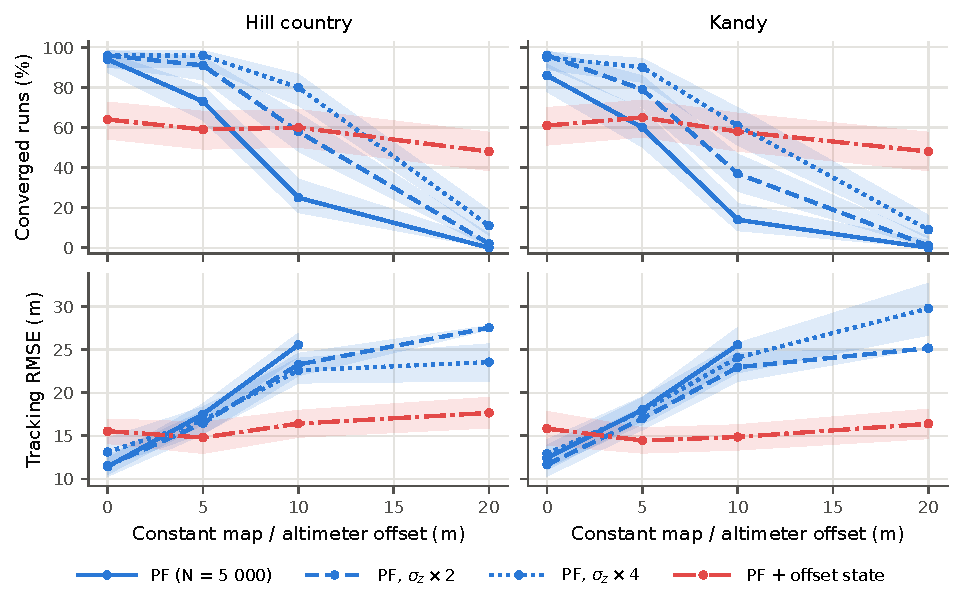
\includegraphics[width=\textwidth]{e4_map_error.pdf}
  \caption{E4: map error --- a spatially correlated field (std 2.4\,m, correlation length 1\,km,
    both assumptions derived from the handbook accuracy) plus a constant offset between the
    measured and the mapped surface. Remedies: measurement std inflated $\times2$ and $\times4$,
    and an extra state for the offset. $M = \EFourRuns$. The EKF is in \cref{tab:e4} only.}
  \label{fig:e4map}
\end{figure}

\paragraph{Map error.} A random map-error field of the size the Copernicus handbook implies is
harmless (\EFourMapErrorHillZeroPfFiveZeroZeroZeroConv\,\% convergence; \cref{fig:e4map}). A
\emph{constant} offset between the measured and the mapped height --- a barometric bias, or a radar
that sees the ground under a canopy the surface model includes --- is not: the nominal filter
converges in \EFourMapErrorHillFivePfFiveZeroZeroZeroConv\,\% of the runs at 5\,m,
\EFourMapErrorHillOneZeroPfFiveZeroZeroZeroConv\,\% at 10\,m and
\EFourMapErrorHillTwoZeroPfFiveZeroZeroZeroConv\,\% at 20\,m, because a profile shifted in height
matches the map best at the wrong place. Inflating $\sigma_z$ fourfold tolerates the offset up
to 10\,m (\EFourMapErrorHillOneZeroPfSzXFourConv\,\%) but not 20\,m
(\EFourMapErrorHillTwoZeroPfSzXFourConv\,\%). Estimating the offset as a fifth state is the only
remedy that still works at 20\,m (\EFourMapErrorHillTwoZeroPfHbiasConv\,\%), and it recovers the
offset itself (mean estimate \EFourHbHillOTwoZeroMean\,m for a true 20\,m; \cref{tab:e4hb}). It
pays for this when there is no offset: \EFourMapErrorHillZeroPfHbiasConv\,\% instead of
\EFourMapErrorHillZeroPfFiveZeroZeroZeroConv\,\%, because with an unknown offset a terrain
profile matches at more places, and the same 5\,000 particles now have to cover five dimensions.
This is a genuine trade-off, not a free improvement.

\paragraph{INS grade.} With an initial bias std of 0.1, 0.3 and 1.0\,m/s the particle filter
converges in \EFourInsGradeHillZeroPointOnePfFiveZeroZeroZeroConv,
\EFourInsGradeHillZeroPointThreePfFiveZeroZeroZeroConv{} and
\EFourInsGradeHillOnePfFiveZeroZeroZeroConv\,\% of the runs (EKF:
\EFourInsGradeHillZeroPointOneEkfConv, \EFourInsGradeHillZeroPointThreeEkfConv,
\EFourInsGradeHillOneEkfConv\,\%) and its tracking error grows with the bias
(\cref{fig:e4ins}): a poor INS makes the terrain do more of the work.

\begin{figure}[t]
  \centering
  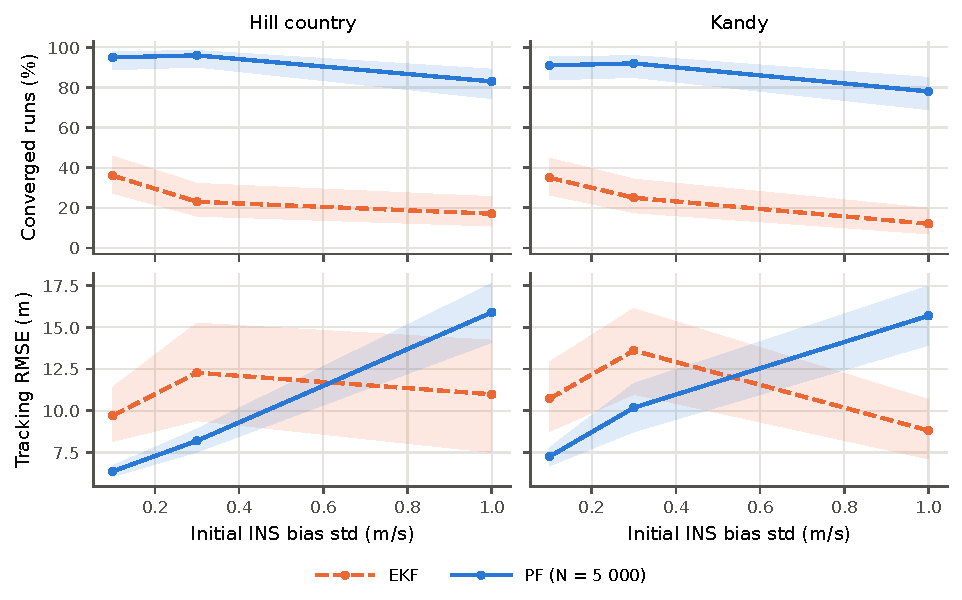
\includegraphics[width=\textwidth]{e4_ins_grade.pdf}
  \caption{E4: INS grade (initial velocity-bias std per axis); $M = \EFourRuns$. Dead reckoning
    never converges and is omitted.}\label{fig:e4ins}
\end{figure}

\begin{table}[t]
  \centering\small
  \caption{E4: offset estimated by the offset-state PF (mean over the final 100\,s, converged
    runs).}\label{tab:e4hb}
  % Generated by scripts — do not edit.
\begin{tabular}{lrrrr}
\toprule
Region & True offset (m) & Converged runs & Mean estimate (m) & Std of error (m) \\
\midrule
Hill country & 0 & 64 & -0.7 & 4.0 \\
Hill country & 10 & 60 & 10.2 & 4.3 \\
Hill country & 20 & 48 & 18.3 & 4.3 \\
Hill country & 5 & 59 & 5.1 & 3.3 \\
Kandy & 0 & 61 & 0.9 & 4.2 \\
Kandy & 10 & 58 & 10.4 & 4.1 \\
Kandy & 20 & 48 & 19.4 & 4.6 \\
Kandy & 5 & 65 & 4.8 & 3.7 \\
\bottomrule
\end{tabular}

\end{table}

\subsection{E5 --- Consistency and the theoretical bound}\label{sec:e5}
\emph{Setup:} the ensemble analysis reuses the E1 runs ($M = \EOneRuns$ per cell); the
per-flight analysis flies five fixed flight plans per region, each $M = 100$ times with fresh
sensor noise and initial error ($\sigma_0 = 500$\,m). The bounds use the true noise of the
simulation (\cref{sec:pcrb}).

\begin{figure}[t]
  \centering
  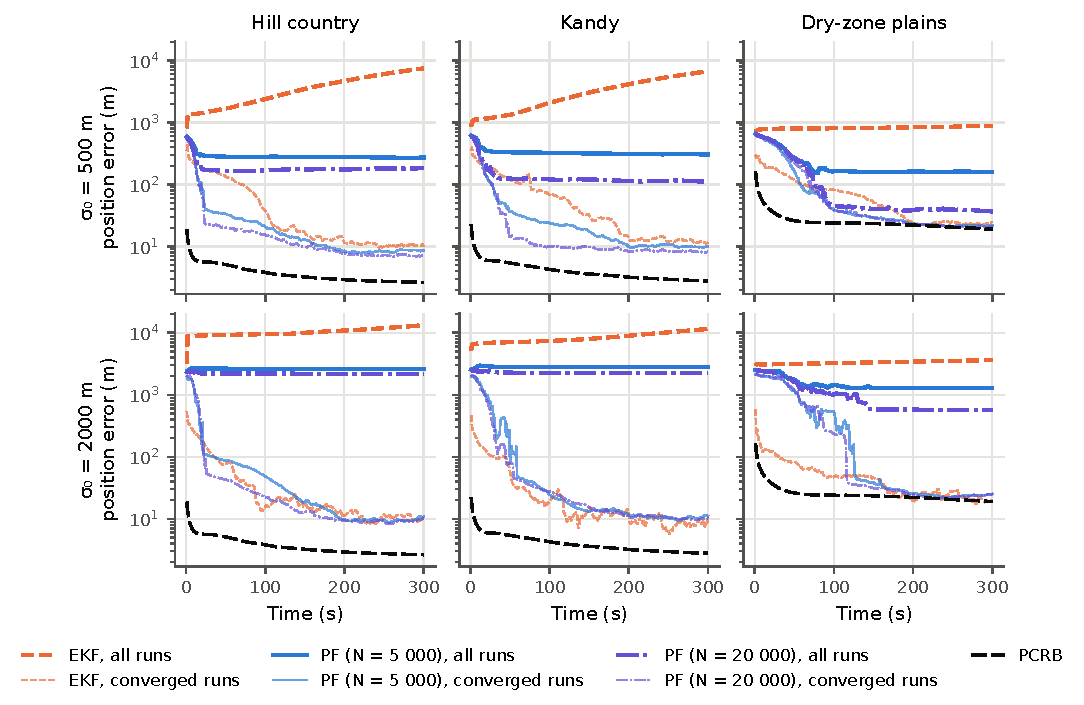
\includegraphics[width=\textwidth]{e5_bound.pdf}
  \caption{E5: RMSE over all runs (thick) and over converged runs (thin) against the ensemble
    PCRB (black), from the E1 runs ($M = \EOneRuns$).}\label{fig:e5bound}
\end{figure}

\paragraph{The bound and ambiguity.} The posterior Cramér--Rao bound is never violated: over all
regions, $\sigma_0$ and filters the all-run RMSE is at least 1.1 times the bound at every time step
(\cref{tab:e5cons}), a useful end-to-end check of the simulation, the filters and the bound. How
far above the bound the filters are depends on ambiguity (\cref{fig:e5bound}). The bound drops to
a few metres within seconds on the hilly regions (\EFiveHillSFiveZeroZeroBound\,m in the tracking
window on the hill country), because it only uses the slope at the true position: it describes a
filter that already knows which hill it is over. With $\sigma_0 = 100$\,m, where false locks do not
occur, the 20\,000-particle PF's all-run RMSE in the tracking window is
\EFiveHillSOneZeroZeroPfTwoZeroZeroZeroZeroBoundRatioAll{} times the bound on the hill country and
\EFivePlainsSOneZeroZeroPfTwoZeroZeroZeroZeroBoundRatioAll{} times on the plains; at $\sigma_0 =
500$\,m the few false locks alone raise the hill-country ratio to
\EFiveHillSFiveZeroZeroPfTwoZeroZeroZeroZeroBoundRatioAll. The gap between the thick and thin
curves in \cref{fig:e5bound} is the price of ambiguity, which no bound based on local slopes can
capture.

\begin{figure}[t]
  \centering
  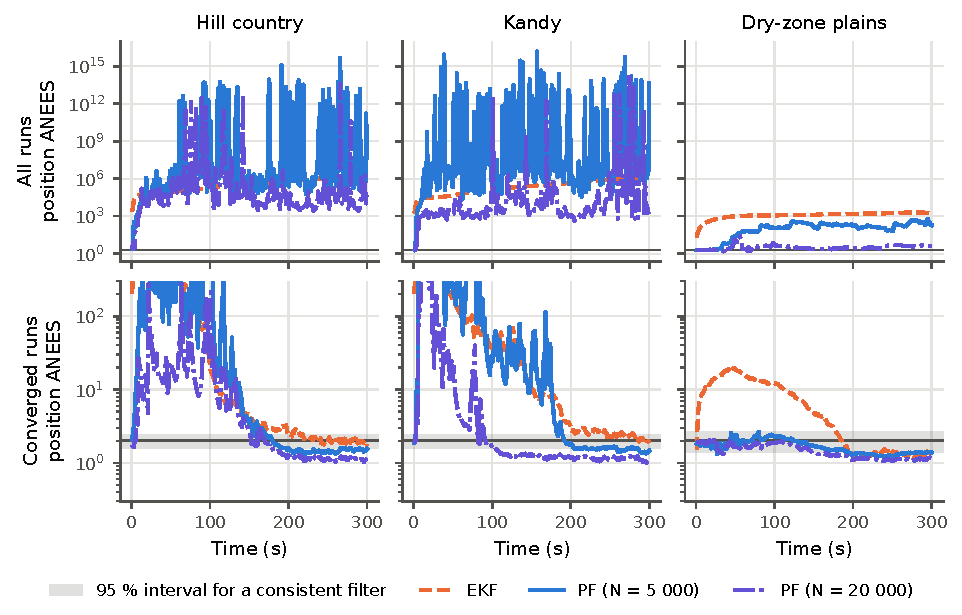
\includegraphics[width=\textwidth]{e5_anees.pdf}
  \caption{E5: position ANEES over all runs (top) and over converged runs (bottom) at
    $\sigma_0 = \EFiveAneesSigma$\,m, with the 95\,\% interval for a consistent filter (grey band;
    $M = \EOneRuns$). Log scale.}\label{fig:e5anees}
\end{figure}

\paragraph{Consistency.} Over all runs the ANEES is meaningless --- up to $10^{15}$ --- because a
falsely locked cloud is tight and far from the truth (\cref{fig:e5anees}, top). In the tracking
window of converged runs the PF is consistent to slightly conservative: ANEES
\EFiveHillSOneZeroZeroPfTwoZeroZeroZeroZeroAneesConv{} at $\sigma_0 = 100$\,m and
\EFiveHillSFiveZeroZeroPfTwoZeroZeroZeroZeroAneesConv{} at 500\,m on the hill country, against a
95\,\% interval of about [\EFiveAneesLo, \EFiveAneesHi], with
\EFiveHillSFiveZeroZeroPfTwoZeroZeroZeroZeroInside\,\% of the individual NEES values inside their
$\chi^2_2$ interval. Values below 2 are expected from the deliberately inflated process noise.
During acquisition, however, even runs that eventually converge have ANEES far above 2: while
most of the weight sits on a wrong mode and a few particles remain near the truth, the weighted
covariance ($\sim$50\,m) understates the error ($\sim$500\,m). A Gaussian consistency measure
simply does not fit a multimodal posterior; the NEES is informative only once the posterior is
unimodal.

\begin{figure}[t]
  \centering
  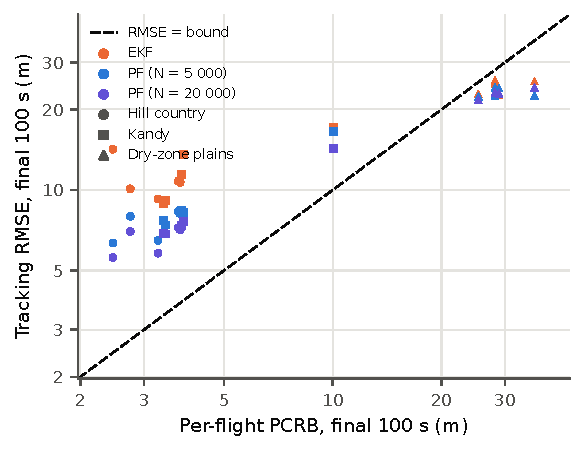
\includegraphics[width=0.6\textwidth]{e5_plans.pdf}
  \caption{E5: tracking RMSE of converged runs against the per-flight PCRB, for five fixed flight
    plans per region ($M = 100$ each, $\sigma_0 = 500$\,m). On the plains the bound is comparable
    to the 50\,m convergence threshold, so restricting the RMSE to converged runs truncates it
    and points fall below the diagonal; the unconditional RMSE never does.}\label{fig:e5plans}
\end{figure}

\paragraph{Why the filters stay above the bound.} Per flight (\cref{fig:e5plans,tab:e5plans}),
the converged 20\,000-particle PF tracks at \EFivePlanHillPfTwoZeroZeroZeroZeroRatio{} times the
bound on the hill country and \EFivePlanKandyPfTwoZeroZeroZeroZeroRatio{} times around Kandy
(medians over the five plans). This gap was tested rather than assumed: a Kalman filter that knows
the true terrain slopes along the path but uses the particle filter's tuning ($\sigma_p = 2$\,m per
step instead of the true $\approx 0.05$\,m) has an actual tracking RMSE of
\EFivePlanHillPfTwoZeroZeroZeroZeroTuned\,m on the hill country --- the mismatched-gain
recursion of \cref{app:mismatch} --- and the particle filter reaches
\EFivePlanHillPfTwoZeroZeroZeroZeroRmse\,m, i.e.\ \EFivePlanHillPfTwoZeroZeroZeroZeroRatioTuned{}
times what its tuning allows (Kandy: \EFivePlanKandyPfTwoZeroZeroZeroZeroRatioTuned). Nearly the
whole factor of two to the bound is the deliberate process-noise inflation, not the particle
approximation. With 5\,000 particles about 20\,\% of Monte Carlo error is added
(\EFivePlanHillPfFiveZeroZeroZeroRatioTuned); the EKF's converged runs are
\EFivePlanHillEkfRatioTuned{} times the tuned limit, because it linearises at its own estimate
rather than at the truth.

\subsection{E6 --- Detecting and recovering from false lock}\label{sec:e6}
\emph{Setup:} the divergence monitor of \cref{sec:monitor} (re-spread fraction $\alpha = 0.5$)
was tuned on separate development seeds ($M = \ESixDevRuns$ per cell; \cref{tab:e6dev}) with a
rule fixed in advance: the best convergence at $\sigma_0 = 2$\,km among settings with at most
5\,\% of runs raising an alarm at $\sigma_0 = 250$\,m. No setting met that constraint (the lowest
was 8\,\%), so --- decided on the development data before the test runs, and recorded as such ---
the setting with the fewest false alarms was taken: window $L = \ESixWindow$, $p_{\mathrm{FA}} =
\ESixPfa$. The test on the main seeds ($M = \ESixTestRuns$) compares, on identical flights, the
plain PF ($N = 5\,000$), the PF with the monitor, the PF with roughening ($K = 0.05$, the value
that worked best in E3) and the PF with both. The monitor against the plain PF is the primary
comparison; the other two were added because E3 had shown roughening to attack the same failure.

\begin{figure}[t]
  \centering
  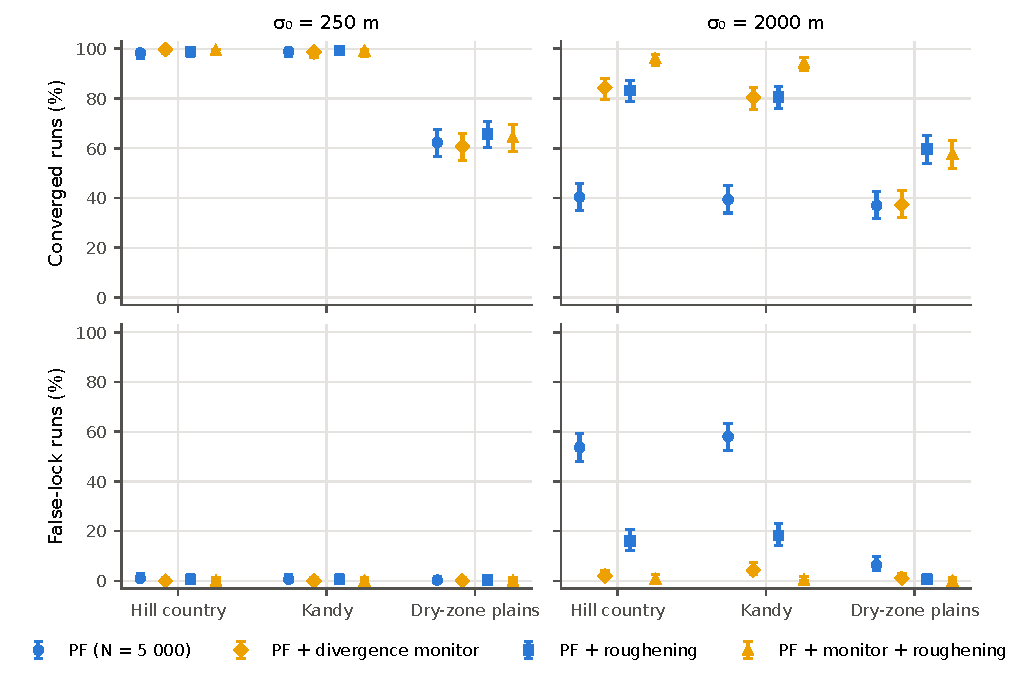
\includegraphics[width=\textwidth]{e6_test.pdf}
  \caption{E6: converged (top) and falsely locked (bottom) runs for the four variants at
    $\sigma_0 = 250$\,m and 2\,km, $M = \ESixTestRuns$ on the main seeds, Wilson 95\,\% intervals.}
  \label{fig:e6}
\end{figure}

The monitor does what it was designed for (\cref{fig:e6,tab:e6}). At $\sigma_0 = 2$\,km on the
hill country it raises convergence from \ESixHillSTwoZeroZeroZeroPfFiveZeroZeroZeroConv\,\% to
\ESixHillSTwoZeroZeroZeroPfMonitorConv\,\% and cuts false lock from
\ESixHillSTwoZeroZeroZeroPfFiveZeroZeroZeroFl\,\% to \ESixHillSTwoZeroZeroZeroPfMonitorFl\,\%
(Kandy: \ESixKandySTwoZeroZeroZeroPfFiveZeroZeroZeroConv\,\% $\to$
\ESixKandySTwoZeroZeroZeroPfMonitorConv\,\%; McNemar $p < 0.001$ on both regions). At
$\sigma_0 = 250$\,m, where it should stay silent, \ESixHillSTwoFiveZeroPfMonitorAlarm\,\% of the
hill-country runs raise an alarm, but convergence is unaffected
(\ESixHillSTwoFiveZeroPfFiveZeroZeroZeroConv\,\% $\to$ \ESixHillSTwoFiveZeroPfMonitorConv\,\%):
keeping half of the cloud means a false alarm costs little. On the plains the monitor changes
nothing (\ESixPlainsSTwoZeroZeroZeroPfFiveZeroZeroZeroConv\,\% vs.\
\ESixPlainsSTwoZeroZeroZeroPfMonitorConv\,\%), as expected: there the filter does not fail by locking
falsely, so there is nothing to detect.

Roughening alone is almost as effective on the hills
(\ESixHillSTwoZeroZeroZeroPfRoughConv\,\%) but leaves more false locks
(\ESixHillSTwoZeroZeroZeroPfRoughFl\,\%), and it is the only variant that helps on the plains
(\ESixPlainsSTwoZeroZeroZeroPfRoughConv\,\%). The two mechanisms are complementary: roughening
prevents locks by keeping hypotheses near the truth alive during acquisition; the monitor recovers
from those that still happen. Together they reach \ESixHillSTwoZeroZeroZeroPfMonitorRoughConv\,\%
(hill country) and \ESixKandySTwoZeroZeroZeroPfMonitorRoughConv\,\% (Kandy) at $\sigma_0 = 2$\,km,
with at most \ESixHillSTwoZeroZeroZeroPfMonitorRoughFl\,\% false locks --- better than the plain
filter with 20\,000 particles in E1 (\EOneHillSTwoZeroZeroZeroPfTwoZeroZeroZeroZeroConv\,\%), at a
quarter of the cost. With roughening, the monitor fires in only
\ESixHillSTwoZeroZeroZeroPfMonitorRoughAlarm\,\% of the hill-country runs instead of
\ESixHillSTwoZeroZeroZeroPfMonitorAlarm\,\%: there are fewer locks to catch.

\subsection{E7 --- Rao-Blackwellisation}\label{sec:e7}
\emph{Setup:} plain PF and RBPF with $N \in \{500, 1\,000, 2\,000, 5\,000\}$ on identical flights,
$\sigma_0 = 1$\,km, $M = \ESevenRuns$ per cell. The two filters cost the same per step at equal
$N$ (\cref{tab:runtime}), so equal $N$ is also equal runtime (\cref{fig:e7rt}).

\begin{figure}[t]
  \centering
  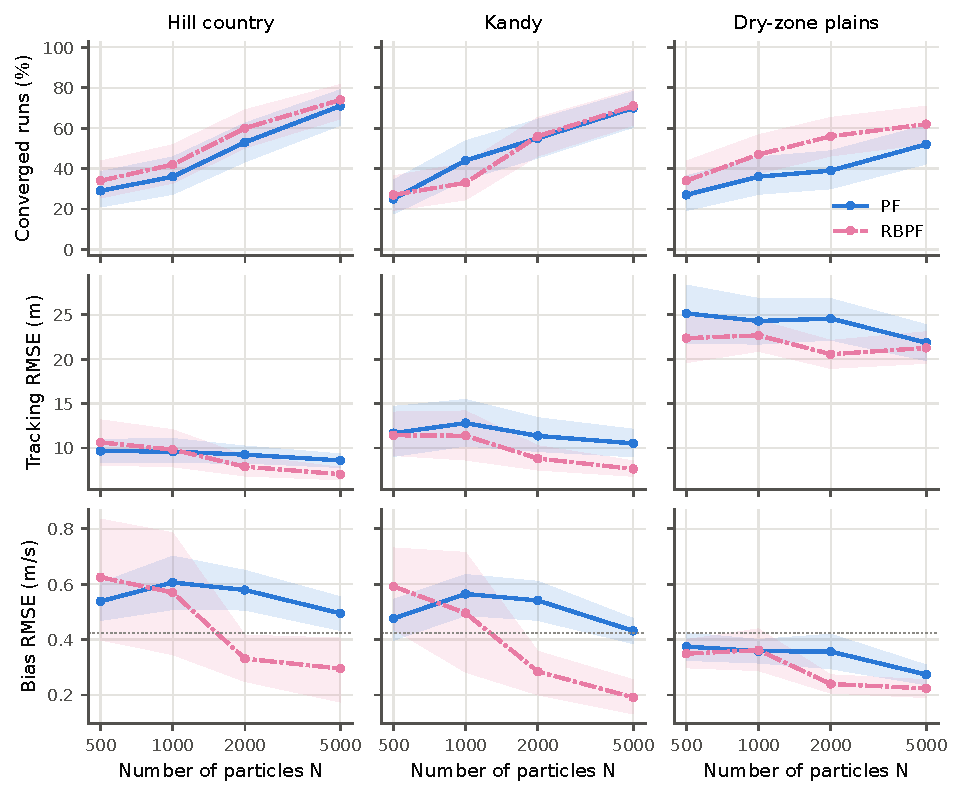
\includegraphics[width=\textwidth]{e7_equal_n.pdf}
  \caption{E7: plain PF vs.\ RBPF at equal particle count: convergence (top), tracking RMSE
    (middle) and RMS error of the INS-bias estimate in the tracking window (bottom; the prior
    alone gives 0.42\,m/s). $M = \ESevenRuns$, $\sigma_0 = 1$\,km, 95\,\% intervals.}\label{fig:e7}
\end{figure}

On the hilly regions the RBPF converges about as often as the plain PF (no significant difference,
McNemar $p \ge 0.09$; \cref{tab:e7}); on the plains it converges more often at every $N$
(\ESevenPlainsRbpfNTwoZeroZeroZeroConv\,\% vs.\ \ESevenPlainsPfNTwoZeroZeroZeroConv\,\% at
$N = 2\,000$, $p = 0.008$). Its clearest advantage is in the quantity it computes exactly
(\cref{fig:e7}): with $N = 5\,000$ on the hill country its bias estimate has an RMS error of
\ESevenHillRbpfNFiveZeroZeroZeroBias\,m/s, against \ESevenHillPfNFiveZeroZeroZeroBias\,m/s for the
plain PF --- whose bias estimate is \emph{no better than the prior} (0.42\,m/s). This is the
well-known impoverishment of an almost static parameter: the bias changes by only 0.002\,m/s
per step, so after repeated resampling all particles' bias values descend from a few ancestors,
and the estimate is roughly one random draw from the prior. The RBPF never samples the bias and
cannot impoverish it. The better bias carries over to tracking: from $N = 2\,000$ the RBPF's
tracking RMSE is lower (\ESevenHillRbpfNFiveZeroZeroZeroTrack{} vs.\
\ESevenHillPfNFiveZeroZeroZeroTrack\,m on the hill country at $N = 5\,000$). With 500 particles
the advantage disappears: each particle's bias filter is then driven by few, noisy position
increments.

\begin{figure}[t]
  \centering
  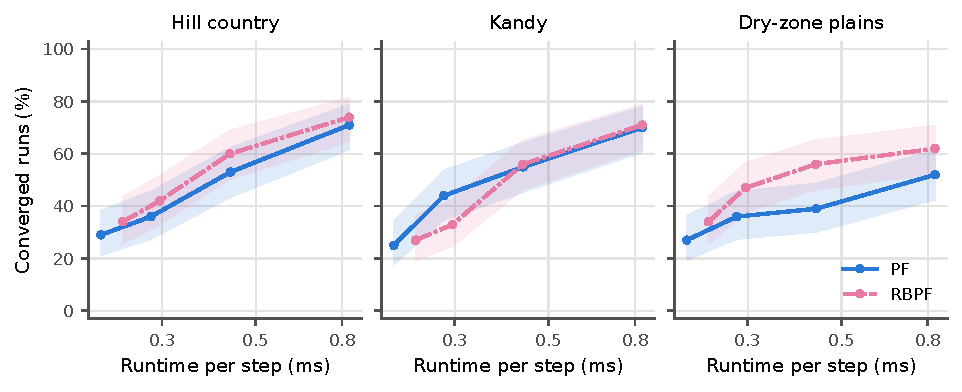
\includegraphics[width=\textwidth]{e7_equal_runtime.pdf}
  \caption{E7: convergence against runtime per step (single-core benchmark); $M = \ESevenRuns$.}
  \label{fig:e7rt}
\end{figure}

\subsection{Illustration}\label{sec:illustration}
\Cref{fig:snapshots,fig:trajectory} show one run, chosen by a fixed rule rather than by eye: the
lowest-index E1 run on the hill country with $\sigma_0 = 2$\,km in which the 20\,000-particle PF
converged after at least 60\,s and the EKF did not. It was re-simulated from its seeds with the
particle cloud recorded, reproducing the saved run exactly. Five seconds after take-off the cloud
has fragmented into clusters along terrain contours --- the multimodal posterior the EKF cannot
represent. By 20\,s it has collapsed onto one tight cluster some 100--150\,m from the truth, a
temporarily wrong mode, and between 60 and 150\,s the measurements move it onto the truth, where
it stays. Meanwhile the EKF confidently follows the wrong slope away from the truth and ends
further off than dead reckoning. An animation of this run (\texttt{report/figures/visuals\_animation.mp4})
is in the repository.

\begin{figure}[t]
  \centering
  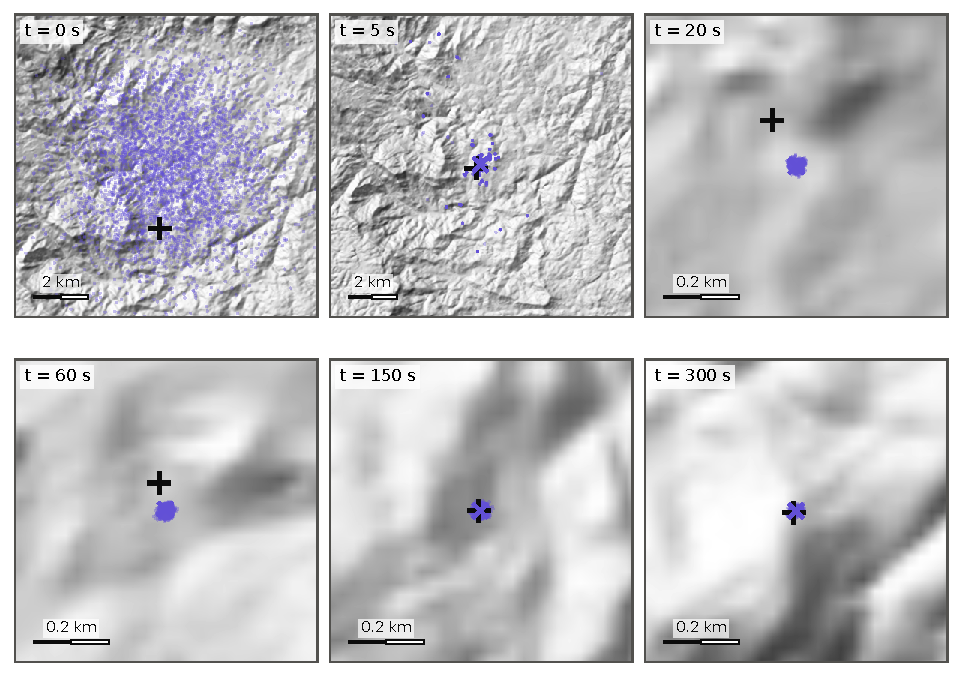
\includegraphics[width=\textwidth]{visuals_snapshots.pdf}
  \caption{Particle cloud (blue, 4\,000 of 20\,000 particles shown) over the hill-country
    hillshade at six instants of the illustrative run; $+$ truth, $\times$ PF estimate. Note the
    changing scale bars.}\label{fig:snapshots}
\end{figure}

\begin{figure}[t]
  \centering
  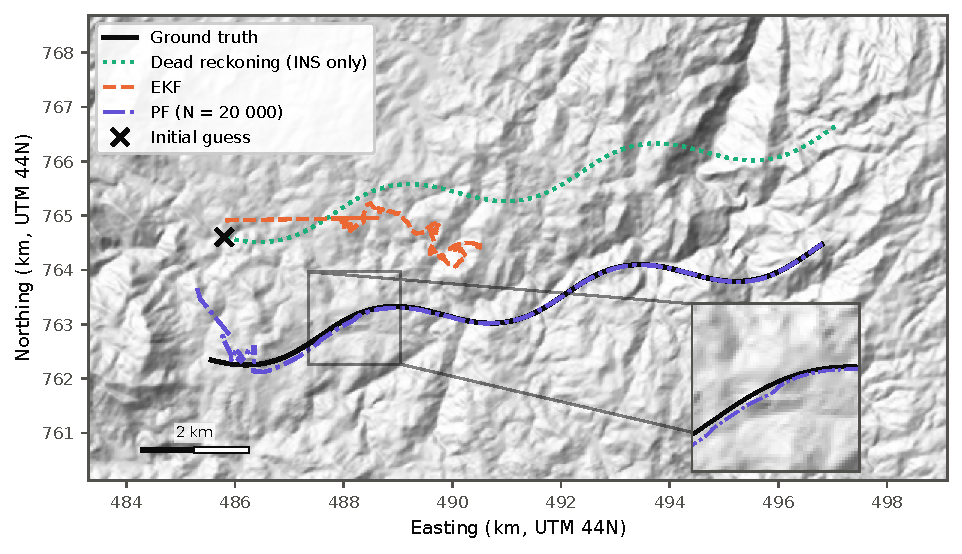
\includegraphics[width=\textwidth]{visuals_trajectory.pdf}
  \caption{Trajectories of the illustrative run; inset: the lock-on of the particle filter
    (20\,s before to 20\,s after its convergence time).}\label{fig:trajectory}
\end{figure}
